% Auto-generated by src/utils/export_paper_artifacts.py
% Drop into a NeurIPS / PhysWorld source file that already loads:
%   \usepackage{booktabs,graphicx,amsmath}
% If compiling this file from the outputs/ directory, figures resolve by basename.

\begin{table}[t]
  \centering
  \small
  \caption{Ablation of AC-JEPA world-model variants. Multi-step open-loop latent rollout MSE ($\downarrow$) at horizons $k\in\{1,5,10,20\}$. Physical-property linear-probe accuracy ($\uparrow$, \%) on stiffness class and frictional contact (contact-quadrant labels). Inference cost is next-step world-model latency: frames per second ($\uparrow$) and wall-clock milliseconds per frame ($\downarrow$). Best result in each column is bold.}
  \label{tab:ac-jepa-ablation}
  \begin{tabular}{lccccccrr}
    \toprule
    & \multicolumn{4}{c}{Rollout MSE $\downarrow$}
      & \multicolumn{2}{c}{Probe acc.\ $\uparrow$ (\%)}
      & \multicolumn{2}{c}{Latency} \\
    \cmidrule(lr){2-5}
    \cmidrule(lr){6-7}
    \cmidrule(lr){8-9}
    Method & $k{=}1$ & $k{=}5$ & $k{=}10$ & $k{=}20$ & Stiffness & Friction & FPS $\uparrow$ & ms/frame $\downarrow$ \\
    \midrule
    Full AC-JEPA (VICReg) & 0.172 & 0.188 & 0.199 & 0.199 & \textbf{37.5} & \textbf{29.2} & 608.5 & 1.64 \\
    Variant A (No Covariance) & 0.286 & 0.362 & 0.494 & 0.338 & 37.5 & \textbf{29.2} & 374.3 & 2.67 \\
    Variant B (MSE-only) & \textbf{0.011} & \textbf{0.063} & \textbf{0.063} & \textbf{0.063} & 35.4 & 22.9 & \textbf{786.8} & \textbf{1.27} \\
    Variant C (Pixel Autoencoder) & 0.108 & 0.106 & 0.106 & 0.106 & \textbf{37.5} & 22.9 & 732.3 & 1.37 \\
    \bottomrule
  \end{tabular}
\end{table}

\begin{figure}[t]
  \centering
  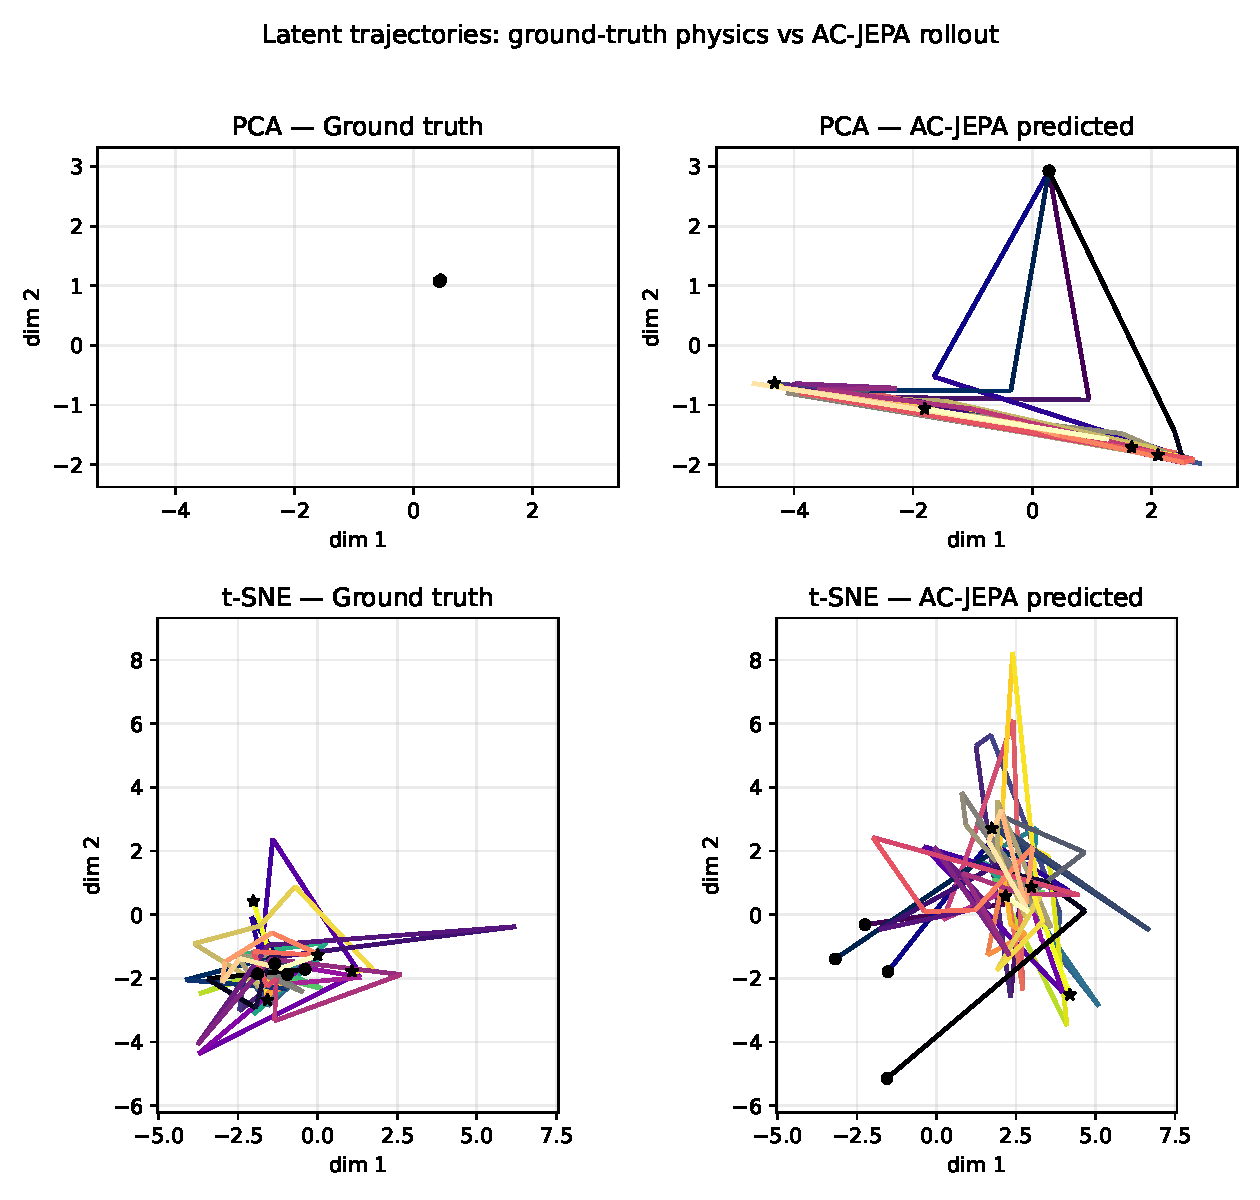
\includegraphics[width=\linewidth]{paper_latent_trajectories.pdf}
  \caption{Side-by-side latent trajectories of ground-truth physical rollouts (target-encoder embeddings $z_{t:t+k}$) versus AC-JEPA open-loop predictions $\hat{z}_{t:t+k}$. Left column: 2D PCA. Right column: t-SNE. Each polyline is one validation episode; color denotes time along the path.}
  \label{fig:ac-jepa-latent-traj}
\end{figure}
